%%%%%%%%%%%%%%%%%%%%%%%%%%%%%%%%%%%%%%%%%
% a0poster Portrait Poster
% LaTeX Template
% Version 1.0 (22/06/13)
%
% The a0poster class was created by:
% Gerlinde Kettl and Matthias Weiser (tex@kettl.de)
% 
% This template has been downloaded from:
% http://www.LaTeXTemplates.com
%
% License:
% CC BY-NC-SA 3.0 (http://creativecommons.org/licenses/by-nc-sa/3.0/)
%
%%%%%%%%%%%%%%%%%%%%%%%%%%%%%%%%%%%%%%%%%

%----------------------------------------------------------------------------------------
%	PACKAGES AND OTHER DOCUMENT CONFIGURATIONS
%----------------------------------------------------------------------------------------

\documentclass[a0,portrait]{a0poster}

\usepackage{multicol} % This is so we can have multiple columns of text side-by-side
\columnsep=100pt % This is the amount of white space between the columns in the poster
\columnseprule=3pt % This is the thickness of the black line between the columns in the poster

\usepackage[svgnames]{xcolor} % Specify colors by their 'svgnames', for a full list of all colors available see here: http://www.latextemplates.com/svgnames-colors

\usepackage{times} % Use the times font
%\usepackage{palatino} % Uncomment to use the Palatino font

\usepackage{graphicx} % Required for including images
\graphicspath{{figures/}} % Location of the graphics files
\usepackage{booktabs} % Top and bottom rules for table
\usepackage[font=small,labelfont=bf]{caption} % Required for specifying captions to tables and figures
\usepackage{amsfonts, amsmath, amsthm, amssymb} % For math fonts, symbols and environments
\usepackage{wrapfig} % Allows wrapping text around tables and figures

\begin{document}

%----------------------------------------------------------------------------------------
%	POSTER HEADER 
%----------------------------------------------------------------------------------------

% The header is divided into two boxes:
% The first is 75% wide and houses the title, subtitle, names, university/organization and contact information
% The second is 25% wide and houses a logo for your university/organization or a photo of you
% The widths of these boxes can be easily edited to accommodate your content as you see fit

\begin{minipage}[b]{0.75\linewidth}
\veryHuge \color{NavyBlue} \textbf{Inference of Chemogenomic Features from Drug-Protein Interactions by EM Algorithm} \color{Black}\\ % Title
\Huge\textit{An Exploration of Global Optimization}\\[2cm] % Subtitle
\huge \textbf{Songpeng Zu, Ting Chen, Shao Li $^{*}$}\\[0.5cm] % Author
\huge Department of Automation, Tsinghua University\\[0.4cm] % University/organization
\Large \texttt{zusongpeng@gmail.com}\\
\end{minipage}
%\
\begin{minipage}[b]{0.25\linewidth}

\includegraphics[width=10cm]{tsinghualogo.png}\\
\end{minipage}

\vspace{1cm} % A bit of extra whitespace between the header and poster content

%----------------------------------------------------------------------------------------

\begin{multicols}{2} % This is how many columns your poster will be broken into, a portrait poster is generally split into 2 columns

%----------------------------------------------------------------------------------------
%	ABSTRACT
%----------------------------------------------------------------------------------------

\color{Navy} % Navy color for the abstract

\begin{abstract}
Gaining insight into chemogenomic drug-target interactions, such as those involving the substructures of synthetic drugs and protein domains, is important in fragment-based drug discovery and drug repositioning. Previous studies evaluated the interactions locally, thereby ignoring the competitive effects of different substructures or domains, but this could lead to high false-positive estimation, calling for a computational method that presents more predictive power.

A statistical model, termed Global optimization-based InFerence of chemogenomic features from drug-Target interactions, or GIFT, is  proposed herein to evaluate substructure-domain interactions globally such that all substructure-domain contributions to drug-target interaction are analyzed simultaneously. Combinations of different chemical substructures were included since they may function as one unit. When compared to previous methods, GIFT showed better interpretive performance, and performance for the recovery of drug-target interactions was good. Among 53 known drug-domain interactions, 81\% were accurately predicted by GIFT. Eighteen of the top 100 predicted combined substructure-domain interactions had corresponding drug-target structures in the Protein Data Bank database, and 15 out of the 18 had been proved. GIFT was then implemented to predict substructure-domain interactions based on drug repositioning. For example, the anticancer activities of tazarotene, adapalene, acitretin and raloxifene were identified. In summary, GIFT is a global chemogenomic inference approach and offers fresh insight into drug-target interactions.
The source codes and results can be found at \\http://bioinfo.au.tsinghua.edu.cn/software/GIFT.

\end{abstract}

%----------------------------------------------------------------------------------------
%	INTRODUCTION
%----------------------------------------------------------------------------------------

\color{SaddleBrown} % SaddleBrown color for the introduction

\section*{Introduction}
Gathering chemogenomic data about protein domains and the chemical substructures of drugs underlying drug-target interactions could foster the development of fragment-based drug discovery, drug repositioning and the understanding of drug-induced side effects, thereby supplementing the network pharmacology methods of target prediction.

However, previous methods were not able to evaluate uncertainty or variance of results, and they also ignored the possible combinations of drug chemical substructures that bind to protein domains as a whole. More importantly, the competitive effects of different substructure-domain interactions have never been considered since prediction has, thus far, been performed locally.

\begin{center}\vspace{1cm}
  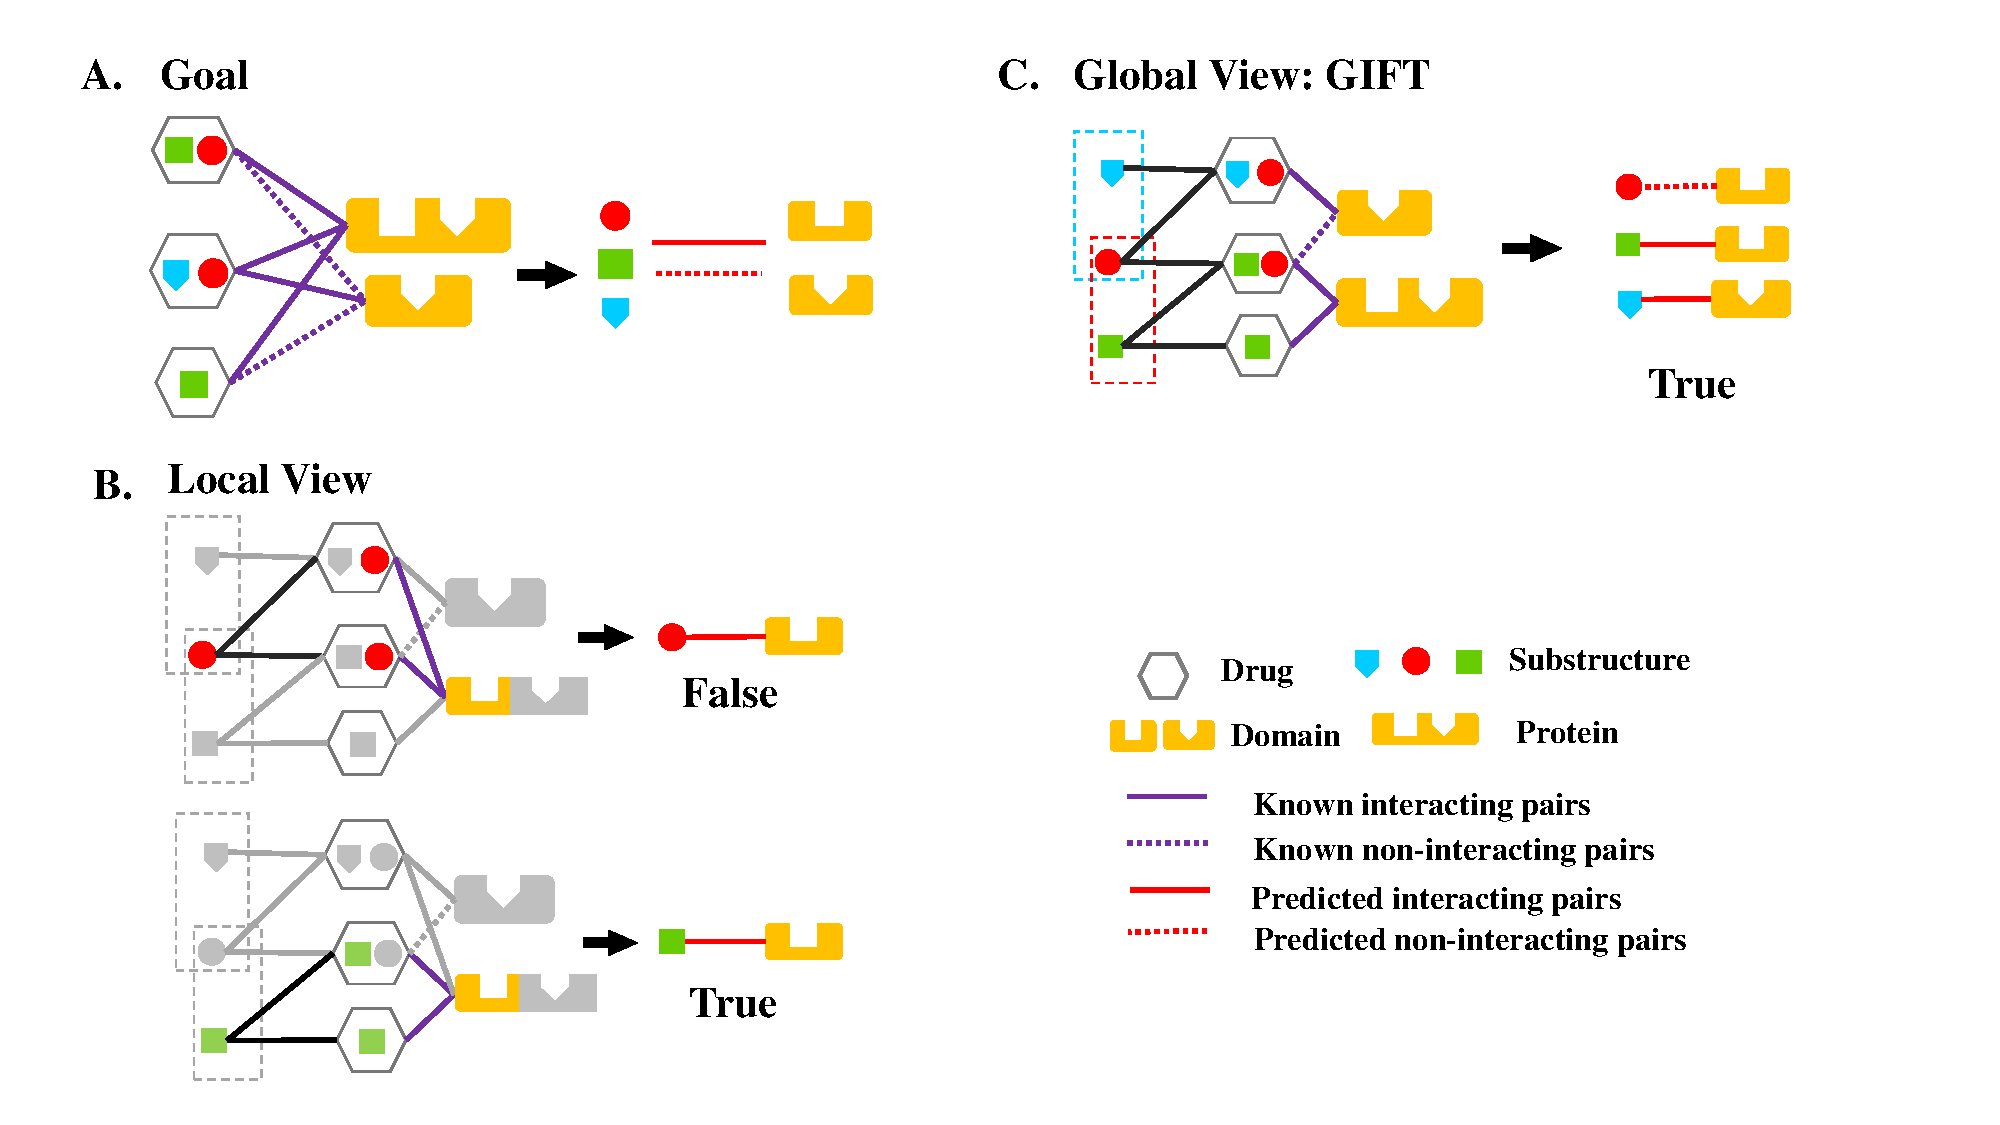
\includegraphics[width=\linewidth]{explains_v2}
\captionof{figure}{\color{Black} Schematic diagram of GIFT. A. The goal of GIFT is to infer the underlying drug substructure-protein domain interactions, given a set of drug-protein interactions. B. The local view of previous approaches that test one pair of substructure-domain at a time while ignoring other substructures or protein domains. C. The global view of GIFT that considers contributions of all substructure-domain pairs to the given set of drug-target interactions.}
\end{center}\vspace{1cm}

%----------------------------------------------------------------------------------------
%	OBJECTIVES
%----------------------------------------------------------------------------------------

\color{DarkSlateGray} % DarkSlateGray color for the rest of the content

%\section*{Main Objectives}
%
%\begin{enumerate}
%\item Infer
%
%\end{enumerate}

%----------------------------------------------------------------------------------------
%	MATERIALS AND METHODS
%----------------------------------------------------------------------------------------

\section*{Materials and Methods}
 A total of 1862 drugs are represented by 881-dimensional chemical substructure binary vectors from PubChem database, and 1554 proteins are represented by 876-dimensional protein domain binary vectors from the Pfam database. 4809 interactions exist between the drugs and the proteins.

%------------------------------------------------

\subsection*{The EM framework of GIFT}


Let $Y_1\ldots Y_T$ denote the T drugs, and $P_1\ldots P_S$ denote the S proteins.Let $Z_1\ldots Z_M$ denote the M drug chemical substructures and let $D_1\ldots D_N$ denote the N protein domains.Let $ZD^{(ij)}$ denote the set of the pairs of chemical substructures and domains from drug $Y_i$ and protein $P_j$ correspondingly. Let $ZD_{mn}$ denote the interaction result between the chemical substructure $D_m$ and the domain $D_n$.$ZD^{(ij)}_{mn} = 1$ if they interact and $ZD^{(ij)}_{mn}=0$ otherwise.Let $YP_{ij}$denotes the interaction result between the drug $Y_i$ and the protein $P_j$. $YP_{ij}=1$ if they interact and $YP_{ij}=0$ otherwise.

For our calculations, it was assumed that i) the interactions of the drug chemical substructures and the protein domains are independent, given a pair of a drug and a protein pair; ii) interactions between a given drug chemical substructure and protein domain would remain unchanged between different pairs of thedrugs and proteins containing them, as shown by
\begin{equation}
\theta_{mn} = Pr(D_{mn}^{(ij)}=1)
\end{equation}
in which $\theta_{mn} = Pr(D_{mn} = 1)$;
iii) drug and the protein will interact if, and only if, one pair of chemical substructures and domains from them interact. Based on these assumptions, we can get
\begin{equation}
Pr(YP_{ij}=1|\theta)=1-\prod_{D_{mn}^{(ij)}}(1-\theta_{mn})
\end{equation}
We include two types of errors in the data of the drug protein interactions: \textit{fp} (false positive rate), in which the drug and the protein do not interact, but are recorded to be interacting, and \textit{fn} (false negative rate) , in which the drug and the protein interact, but are not recorded. Let $O_{ij}$ be the result of observed interaction between drug $Y_i$ and protein $P_j$:$O_{ij}=1$ if the interaction is observed and $O_{ij}=0$ otherwise.\\Then
\begin{eqnarray}
\textit{fp}=Pr(O_{ij}=1|YP_{ij}=0),
\textit{fn}=Pr(O_{ij}=0|YP_{ij}=1)
\end{eqnarray}
Both \textit{fn} and \textit{fp} are fixed in GIFT.

And the probability for the observed interaction between drug $Y_{i}$ and the protein $P_{j}$ is
\begin{equation}
\begin{aligned}
Pr(O_{ij}&=1|\theta)=(1-\textit{fn})Pr(YP_{ij}=1|\theta)+\textit{fp}\cdot Pr(YP_{ij}=0|\theta)
\end{aligned}
\end{equation}
The log likelihood function is followed
\begin{equation}
\begin{aligned}
l(\theta)&=log(Pr(O|\theta))\\
\end{aligned}
\end{equation}

Let $A_m$ be the set of drugs containing the chemical substructure $Z_m$ and let $A_n$ be the set of proteins containing the domain $D_n$. Let $N_{mn}$ be the total number of pairs between $A_m$ and $A_n$. The EM algorithm as follows:\\
E Step:
\begin{equation}
  \begin{aligned}
    E(D_{mn}^{(ij)}|O,\theta^{(t-1)})
    &=\frac{\theta_{mn}^{(t-1)}(1-\textit{fn})^{O_{ij}}\textit{fn}^{1-O_{ij}}}{Pr(O_{ij}|\theta^{(t-1)})}
  \end{aligned}
\end{equation}
M Step:
\begin{equation}
\begin{aligned}
\theta_{mn}^{(t)}
&=\frac{1}{N_{mn}} \sum_{i,j: Zm\in Y_i, Dn\in P_j}E(D_{mn}^{(ij)}|O_{ij},\theta^{(t-1)})\\
%&=\frac{1}{N_{mn}}\sum_{i,j: Zm\in Y_i, Dn\in P_j}\frac{\theta_{mn}^{(t-1)}(1-\textit{fn})^{O_{ij}}\textit{fn}^{1-O_{ij}}}{Pr(O_{ij}|\theta^{(t-1)})}
\end{aligned}
\end{equation}
\section*{Results}

Following 5-fold cross validation procedure, we compared GIFT with previous methods, namely, L1-log, L1-SVM, SCCA and the association method, based on their performance for recovery of drug-target interactions. The association method was a naive approach to inference of  substructure-domain interactions. The area under the ROC curve (AUC) of the association method is 0.72 (data not shown). Based on the AUC (See Table 1), GIFT performed better than the association method, L1-Log method, as well as SCCA, and it was comparable to L1-SVM for predicting drug-protein interactions.
\begin{center}\vspace{1cm} % Left or right alignment is specified in the first bracket, the width of the table is in the second
\begin{tabular}{l l l l l}
\toprule
\textbf{Ratio} & \textbf{GIFT} & \textbf{L1-Log} & \textbf{L1-SVM} & \textbf{SCCA}\\
\midrule
1 & 0.835 & 0.829 & 0.830 & 0.798 \\
5 & 0.847 & 0.838 & 0.855 & 0.798 \\
\bottomrule
\end{tabular}
\captionof{table}{\color{Black} Performance of recovery of drug-target interactions. The values are the mean areas under the ROC curves. Ratio is the proportion of negative samples over the total number of training samples.}
\end{center}\vspace{1cm}

%#\begin{center}\vspace{1cm}
%#\begin{tabular}{l l l l}
%#\toprule
%#\textbf{Treatments} & \textbf{Response 1} & \textbf{Response 2} \\
%#\midrule
%#Treatment 1 & 0.0003262 & 0.562 \\
%#Treatment 2 & 0.0015681 & 0.910 \\
%#Treatment 3 & 0.0009271 & 0.296 \\
%#\bottomrule
%#\end{tabular}
%#\captionof{table}{\color{Green} Table caption}
%#\end{center}\vspace{1cm}
GIFT was then evaluated for its performance in predicting drug-domain interactions. The prediction of drug-domain interactions were followed Equation 2 in Methods, and each domain was treated as one protein. A drug and a protein domain were predicted to interact if the score given by GIFT was larger than zero.
81\% of the 53 known drug-domain interactions could be predicted by GIFT. The representative results were shown in Figure 2.

\begin{center}\vspace{1cm}
  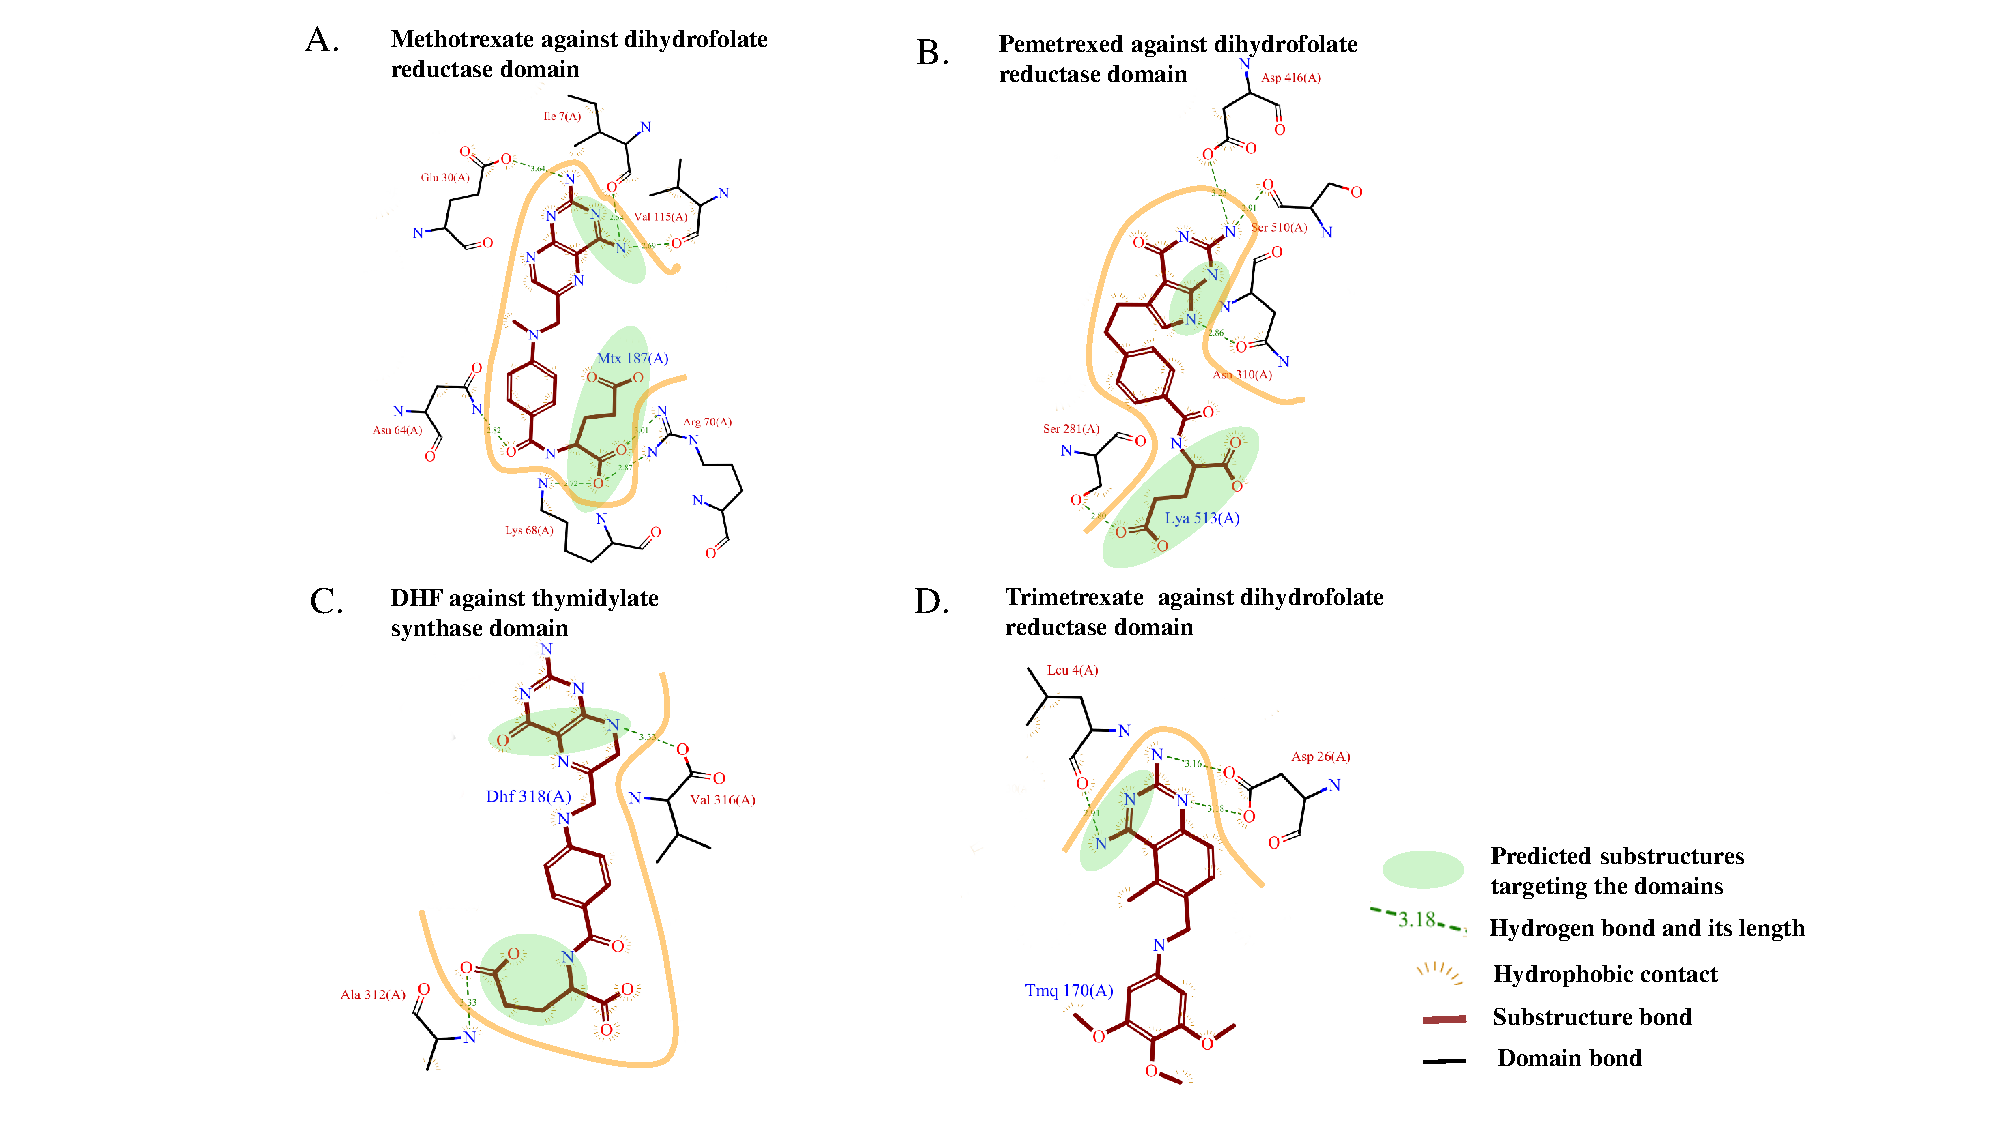
\includegraphics[width=\linewidth]{ligplot_5}
\captionof{figure}{\color{Black} Examples of the substructure-domain interactions validated from the Protein Data Bank database: (A) PDB entry 1u70, (B) PDB entry 3k2h, (C) PDB entry 1lcb, (D) PDB entry 1bzf. Dark grey: the drugs. Black: the amino acids. All the figures are generated by LigPlot.}
\end{center}\vspace{1cm}

%----------------------------------------------------------------------------------------
%	CONCLUSIONS
%----------------------------------------------------------------------------------------

\color{SaddleBrown} % SaddleBrown color for the conclusions to make them stand out


%\begin{itemize}
%\item Pellentesque eget orci eros. Fusce ultricies, tellus et pellentesque fringilla, ante massa luctus libero, quis tristique purus urna nec nibh. Phasellus fermentum rutrum elementum. Nam quis justo lectus.
%\item Vestibulum sem ante, hendrerit a gravida ac, blandit quis magna.
%\item Donec sem metus, facilisis at condimentum eget, vehicula ut massa. Morbi consequat, diam sed convallis tincidunt, arcu nunc.
%\item Nunc at convallis urna. isus ante. Pellentesque condimentum dui. Etiam sagittis purus non tellus tempor volutpat. Donec et dui non massa tristique adipiscing.
%\end{itemize}

\color{DarkSlateGray} % Set the color back to DarkSlateGray for the rest of the content

%----------------------------------------------------------------------------------------
%	FORTHCOMING RESEARCH
%----------------------------------------------------------------------------------------

%\section*{Forthcoming Research}
%
%Vivamus molestie, risus tempor vehicula mattis, libero arcu volutpat purus, sed blandit sem nibh eget turpis. Maecenas rutrum dui blandit lorem vulputate gravida. Praesent venenatis mi vel lorem tempor at varius diam sagittis. Nam eu leo id turpis interdum luctus a sed augue. Nam tellus.
%
 %----------------------------------------------------------------------------------------
%	REFERENCES
%----------------------------------------------------------------------------------------
%\nocite{*} % Print all references regardless of whether they were cited in the poster or not
%\bibliographystyle{plain} % Plain referencing style
%\bibliography{sample} % Use the example bibliography file sample.bib

%\section*{References}
\begin{thebibliography}{}
\bibitem[1]{Songpeng}Zu,S., Chen,T., Li,S. (2015) Global Optimization-based Inference of Chemogenomic Features from Drug-Target Interactions. \textit{Bioinformatics}, \textit{Online}
\bibitem[2]{Tabei2012} Tabei,Y. \textit{et~al}. (2012) Identification of chemogenomic features from drug--target interaction networks using interpretable classifiers. \textit{Bioinformatics}, \textbf{28}, i487-i494.
%\bibitem[3]{Zhao and Li} Zhao,S. and Li,S. (2010) Network-based relating pharmacological and genomic spaces for drug target identification. \textit{Plos One}, \textbf{5},e11764.
\end{thebibliography}
%----------------------------------------------------------------------------------------
%	ACKNOWLEDGEMENTS
%----------------------------------------------------------------------------------------

%\section*{Acknowledgements}
%We thank Dr. Felix A Kruger at University of Cambridge for helpful discussion.

%----------------------------------------------------------------------------------------

\end{multicols}
\end{document}